---
id: tkz-euclide-ejemplo-59
title: "Hexágono regular"
description: "Creación de un hexágono regular"
keywords: [poligono, hexagono, taller3]
tags: [tkzDefRegPolygon,tkzDrawPolygon]
sort: 59
---
\documentclass[tikz,border=2mm]{standalone}
\usepackage{xcolor}
\usepackage{tkz-base}
\usepackage{tkz-euclide}

\begin{document}
    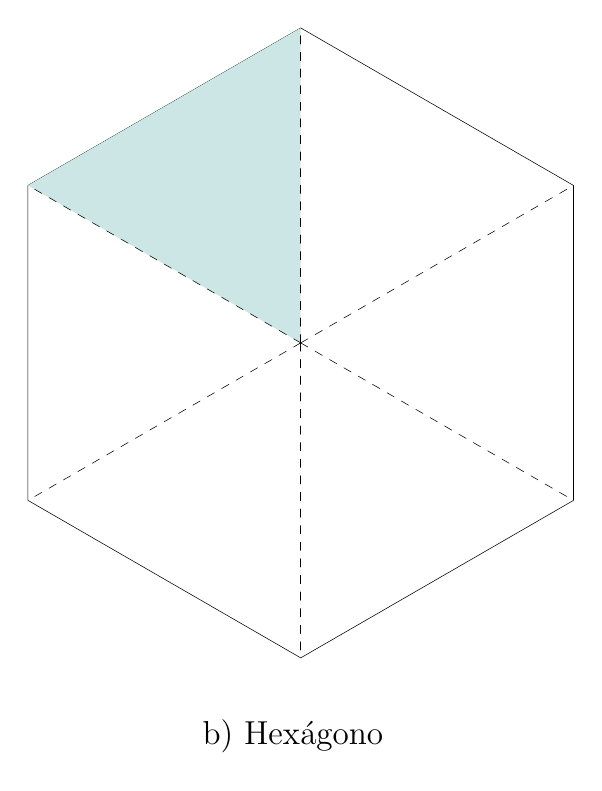
\begin{tikzpicture}
        % Paso 1: Define un punto central y uno del perímetro        
        \tkzDefPoint(13,5){O} % centro
        \tkzDefPoint(13,1){C} % vértice perimetral   

        % Paso 2: Define polígono regular de 6 lados
        % con centro O y punto perimetral C
        % con vêrtices llamaodos Q1,Q2,...,Q6.
        \tkzDefRegPolygon[center,sides=6,name=Q](O,C)

        % Paso 3: Dibuja el hexágono
        \tkzDrawPolygon(Q1,Q...,Q6)

        % Paso B6: Rellena el triángulo O-Q4-Q5 de color turquesa
        \tkzFillPolygon[fill=teal!20](O,Q4,Q5)
        
        % Paso 4: Dibuja un segmento punteado entre el centro y
        % cada uno de los vertices del hexágono
        \foreach \j in {1,...,6} { \tkzDrawSegment[dashed](O,Q\j)}

        % Paso 5: Coloca una leyenda debajo de la figura
        \tkzText(12.9,0){\large{b) Hexágono}}        
    \end{tikzpicture}
\end{document}